%%%%%%%%%%%%%%%%%%%%%%%%%%%%%%%%%%%%%%%%%%%%%%%%%%%%%%%%%%%%%%%%%%%%%%%%
%                                                                      %
%     File: Thesis_Architecture.tex                                %
%     Tex Master: Thesis.tex                                           %
%                                                                      %
%                                                                      %
%%%%%%%%%%%%%%%%%%%%%%%%%%%%%%%%%%%%%%%%%%%%%%%%%%%%%%%%%%%%%%%%%%%%%%%%

\chapter{Architecture of the solution}
\label{chapter:architecture}


%%%%%%%%%%%%%%%%%%%%%%%%%%%%%%%%%%%%%%%%%%%%%%%%%%%%%%%%%%%%%%%%%%%%%%%%
\section{Overview}
\label{section:overview}

As discussed before, The idea is to compare current technologies (Web Services, REST, XML, JSON) with new solution. This solution is a new programming technology alternative current solutions. Basically, this is an alternative to text-based data description (XML and JSON) technologies, for document sharing or service invocation, between two completely different systems. Following sections will explain about how being implemented the interoperability, primitive data formats and solution of binary level compliance and comformance.
%%%%%%%%%%%%%%%%%%%%%%%%%%%%%%%%%%%%%%%%%%%%%%%%%%%%%%%%%%%%%%%%%%%%%%%%

\section{Binary Format}
\label{section:binary}

One of ideas in this technology is using binary format instead of using text or other formats. Because binary is faster to write, communicate and read. When serialization or deserialization performance is compared with binary, XML and JSON, it is easily seen that binary format gives faster speed than the others especially with large data\citep{binary:2016:Online}.\\

On the other hand, using text is far more flexible. Textual representation leads parsing overheads. Messages received are parsed directly in binary, much faster than text parsing. The binary representation provides native support for binary data, has a smaller length and is faster to parse.\\

Defining a binary format which messages are serialized on send and recovered on reception. For binary format using TLV (Tag, Length and Value) binary markup\citep{asn1:opt}, array of bytes are used with each resource serialized in a tag (a byte codifying each resource type), size, name (only on structure and resource components) and value (the actual sequence of bytes resulting from serializing the resource).\\

The binary format used to serialize the resources with TLV (Tag, Length and Value) binary markup as in Table \ref{tab:tvl}. This supports the direct integration of binary information but also facilitates parsing, since each resource, primitive or structured. Binary message format resulting from compilation of the source program and that uses self-description information and only when needed. This allow us maintaining all the information necessary to communicate in a standard and platform independent way.\\


\begin{table}
\centering
\begin{tabular}{ p{5.50cm} p{5.50cm} }
\toprule
\multicolumn{1}{l}{\textbf{Format}} & \textbf{Definition}\\
\midrule
\textbf{Type}  &  A binary code, which indicates the kind of field that this part of the message represents.\\
\textbf{Length} & The size of the value field in bytes \\
\textbf{Value} & Variable-sized series of bytes which contains data for this part of the message.\\

\bottomrule
\end{tabular}
\caption[TLV format (Type-length-value).]{TLV format (Type-length-value).}
\label{tab:tvl}
\end{table}


As long as controlling the serialization format, the serialization can be performed in one language and the
deserialization in another. The binary format is always the result of serializing data in each language, with a tag, the number of bytes that follow and the serialized content. Recovering the serialized data is simply testing the tag to find the data type and then using the number of bytes and the serialized content.\\

Let’s demonstrate this with an example, so as seen in the example of Chapter \ref{chapter:interoperability} that explain interaction between Android mobile phone and .Net weathercast provider. Your phone has an application that written in Java that send query message to .Net weathercast provider and displaying result regarding the respond from .Net weathercast provider.\\

The procedure starts by serializing query message to the binary format in Java. In this case, application in your phone will create binary message instead of XML or JSON to send weathercast provider as in Listing ~\ref{lst:SILserialize}
\begin{lstlisting}[caption=Creating serialized binary Message, label=lst:SILserialize]

  public static void main(String[] args)  {

       Weather w = new Weather();
       w.country="Portugal";
       w.city="Lisbon";
       Message msg = new Message(w);
       byte[] msgToSend =  msg.SeriliazeBinary();
       string response = clientEndPoint.sendMessage(msgToSend);
   }

\end{lstlisting}

Creating a binary message will be similar to TLV (Tag, Length and Value) binary markup idea. Reagarding the code in Listing ~\ref{lst:SILserialize}, the provided binary will be as in Listing ~\ref{lst:SILbinary}.

\begin{lstlisting}[caption=Creating serialized binary Message, label=lst:SILbinary]

[@C1, 3, 0, 0, 0, 7, 0, 0, 0, 7, 0, 0, 0, 8, 0, 0, 0, 8, 99, 111, 117, 110, 116, 114, 121, 80, 111, 114, 116, 117, 103, 97, 108@C, @B1, 3, 0, 0, 0, 4, 0, 0, 0, 4, 0, 0, 0, 6, 0, 0, 0, 6, 99, 105, 116, 121, 76, 105, 115, 98, 111, 110@B, @A1, 3, 0, 0, 0, 4, 0, 0, 0, 4, 0, 0, 0, 0, 0, 0, 0, 0, 100, 97, 116, 101@A]

\end{lstlisting}

Weather object in Listing ~\ref{lst:SILserialize} is serialized by its primitive elements. So in Figure ~\ref{fig:bianryprim}, it can be seen that how first primitive element of weather object, which is, country element is been serialized to binary.

\begin{figure}[!htb]
  \centering
  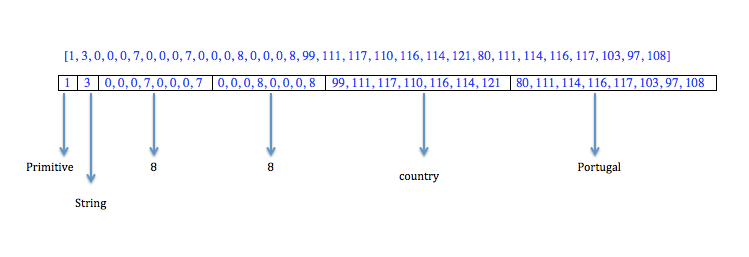
\includegraphics[width=0.9\textwidth]{Figures/binaryrep2.png}
  \caption[Binary representation of primitive resource.]{Binary representation of primitive resource.}
  \label{fig:bianryprim}
\end{figure}

Equation ~\ref{eq:isMandatory} tells that serialization starts with checking if the object is primitive or structure. After that step, equation ~\ref{eq:FieldType} informs you with type of primitive object. In that case it is String object and then next part of binary (equation ~\ref{eq:FieldNameLenght}) informs about primitive field name length, so here, name of the primitive field is “country” and its size is 7. Next part of binary (equation ~\ref{eq:FieldValueLenght}) is field value length, which is “Portugal”, and its size is 8. Since size of field name and value is known, They can be converted to binary. Lastly, equation ~\ref{eq:FieldName} and equation ~\ref{eq:Value} tell us name of the field and value of field.
\begin{subequations}
    \begin{equation}
    1
    \label{eq:isMandatory}
    \end{equation}
    \begin{equation}
    3
    \label{eq:FieldType}
    \end{equation}
    \begin{equation}
    0, 0, 0, 7, 0, 0, 0, 7
    \label{eq:FieldNameLenght}
    \end{equation}
    \begin{equation}
    0, 0, 0, 8, 0, 0, 0, 8
    \label{eq:FieldValueLenght}
    \end{equation}
    \begin{equation}
    99, 111, 117, 110, 116, 114, 121
    \label{eq:FieldName}
    \end{equation}
    \begin{equation}
    80, 111, 114, 116, 117, 103, 97, 108
    \label{eq:Value}
    \end{equation}
\label{eq:NavierStokes}%
\end{subequations}

Creating binary is implemented with following rules:

\begin{itemize}
\item 	An integer is always 64 bits, with each byte serialized in sequence. The receiver will recover the integer in the same way.
\item 	Booleans can use just two different tags. There is no size or content, since the tag says it all needed information.
\item 	Strings use a UTF-8 encoding, since it is already byte oriented.
\item 	Structures. Sequence of fields, in which, for each field, you should include: name (a string) and the component proper (serialized according to its type of resource)
\end{itemize}

Objects with variables should be serialized to a compound data (composed of inner data). This means having a compound data type, with its own tag, and inner components serialized according to their own data type (composition can be recursive). This is always recoverable at the receiver, with advantage of the tag.

%%%%%%%%%%%%%%%%%%%%%%%%%%%%%%%%%%%%%%%%%%%%%%%%%%%%%%%%%%%%%%%%%%%%%%%%
\section{Asymmetric interoperability}
\label{section:AsymmetricInteroperability}

In the new implemented solution, it is showed that how interaction is stil possible with only a partial knowledge of types, as long as the characteristics actually used are included (partial interoperability). This is a way of getting closer to solving the fundamental integration problem, by reducing coupling to what is actually required. Coupling is bad, but without it no interaction is possible. The goal in that thesis is to minimize it as much as
possible, down to the minimum level that ensures the level of interaction required by the resources to integrate.\\

In this solution, a different approach will be showed, based on compliance. Messages do not obey some external schema. Each message has one specific value which are structured or primitive with its own exclusive schema that is nothing more than a self-description, without the value variability that a type exhibits. This value and its description can be validated against an infinite number of schemas, those that have this particular value included in the set of their instances.\\
\begin{figure}[!htb]
 \centering
 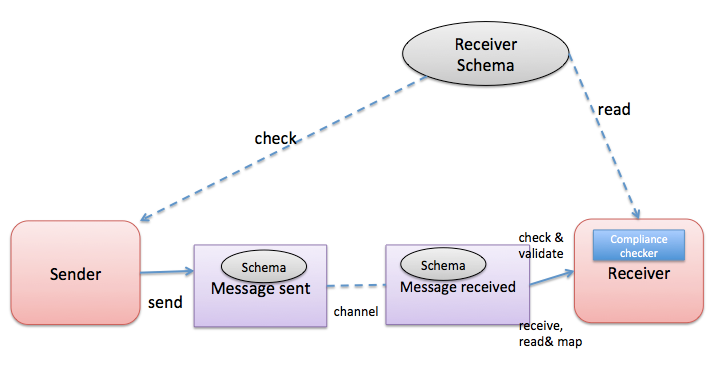
\includegraphics[width=0.9\textwidth]{Figures/asyc.png}
 \caption[Asymmetric interoperability.]{Asymmetric interoperability.}
 \label{fig:Asymmetric}
\end{figure}

The receiver in Figure ~\ref{fig:Asymmetric} exposes a schema that defines the values it is willing to accept.
When a message is received, its internal schema is checked against the receiver’s own schema. If it complies which means satisfies all the requirements of the receiver’s schema, the message can be accepted and processed. The advantage of this is that a resource can send a message to all the resources with schemas that the message complies with and, conversely, a resource can receive messages from any resource that sends messages compliant with its receiving schema. In other words, coupling occurs only in the characteristics actually used by messages and not in all the characteristics of the schemas used to generate the message or to describe the service of the receiving resource. Since the schemas of the message and of the receiver are not agreed beforehand, they need to be checked structurally. Resources of primitive types have predefined compliance rules. Structured resources are compared by the names of components (regardless of order of declaration or appearance) and (recursively) by the compliance between structured resources with matching names. Since the order of appearance of named component resources may different in the message and in the receiving schema, there is the need to map one onto the other. This is a form of polymorphism that increases the range of applicability of both sender and receiver, constituting a means to reduce coupling to only what is actually used. Sender and receiver no longer need to be designed for each other but, as long as compliance is ensured, one resource can replace another. In this case, what is involved is conformance between the replacement and the resource replaced, stating that the former supports all the characteristics supported by the latter. When a resource is able to interact with another, although not entirely interoperable with it, it means that there is partial interoperability.

\begin{figure}[!htb]
 \centering
 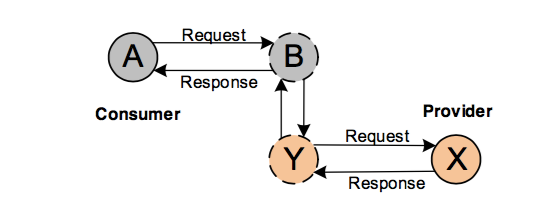
\includegraphics[width=0.9\textwidth]{Figures/partial.png}
 \caption[Partial interoperability, based on compliance and conformance.]{Partial interoperability, based on compliance and conformance.}
 \label{fig:Partial}
\end{figure}

Figure ~\ref{fig:Partial} illustrates these concepts and differentiates compliance from conformance. It also describes complete transactions, with both request and response. The interacting resources now perform the roles of consumer who makes the request and provider, with sender and receiver roles reversed from request to response.\\

Interoperability of a consumer with a provider is possible by satisfying the following properties:

Compliance\citep{compliance:def} which means that the consumer must satisfy (comply with) the requirements established by the provider to accept requests sent to it, without which these cannot be honored.

Conformance\citep{comformance:def2} which means that the provider must fulfill the expectations of the consumer
regarding the effects of a request (including eventual responses), therefore being able to take the form
of (to conform to) whatever the consumer expects it to be.


In full interoperability, the consumer can use all the characteristics that the provider exposes. This is what happens when schemas are shared. In partial interoperability, the consumer uses only a subset of those characteristics, which means that compliance and conformance need only be ensured for that subset. These properties are not commutative (e.g., if P complies with Q, Q does not necessarily comply with P), since the
roles of consumer and provider are different and asymmetric by nature, but are transitive (e.g., if P complies with Q and Q complies with R, then P complies with R)

In Figure ~\ref{fig:Partial} , a resource A, in the role of consumer, has been designed for full interoperability
with resource B, in the role of provider. A uses only the characteristics that B offers and B offers only the
characteristics that A uses. Let's assume that the provider of A is needed to change to resource X, which has been designed for full interoperability with resource Y, in the role of consumer. The problem is that A was designed to interact with provider B and X was designed to expect consumer Y. This means that, if you use resource X as a provider of A, B is how A views provider X and Y is how X views consumer A. Ensuring that A is interoperable with X requires two conditions such as Compliance and Conformance.
For Compliance; B must comply with Y. Since A complies with B and Y complies with X, this means that A complies with X and, therefore, A can use X as if it were B, as it was designed for.
For Conformance: Y must conform to B. Since X conforms to Y and B conforms to A, this means that X conforms to
A and, therefore, X can replace (take the form of) B without A noticing it.
 Partial interoperability has been achieved by subsumption, with the set of characteristics that A uses as a subset of the set of characteristics
offered by X. This inclusion relationship, without changing characteristics, is similar in nature to the
inheritance-based polymorphism supported by many programming languages, but here it applies to a distributed context. It constitutes the basis for transitivity in compliance and conformance, as well as the mechanism to reduce coupling between two resources to the minimum required by the application.


%\section{Compliance and Conformance}
%\label{section:Compliance}

%The other idea in this technology is using compliance and conformance instead of sharing the same schema. There are no schemas or data types that need to be shared or agreed upon beforehand. This means that two partners will be able to communicate as long as the sender complies with receiver which follow what the receiver requires and the receiver conforms to what the sender expects (supports all the features that the sender requires), just in the features actually invoked by the sender.\\

%When a resource receives a message, it tries to match it against the type of the input parameter of each of its operations. If one is found, the message received is partially assigned to that argument and the operation invoked. Partial assignment means that the input parameter is created first, then each matching component (by name) of the message is assigned to the parameter. This means that some components of the message can be ignored and some components of the argument may stay unassigned (these are the components that do not match). If all non-optional components in the argument are matched, there is compliance, the matching components of the message are assigned to those of the argument with the same name and those that do not match are ignored. Thus the designation partial assignment.\\

%Using the simple matching that we described above to avoid complexity in the implementation and  still achieve
%interoperability based on compliance and show that two different messages can still match a given operation's argument.

Referring again the example in Chapter \ref{chapter:introduction} that demonstrate interaction between Android mobile phone and .Net weathercast provider. Now let's demonstrate how it works with a new implemented solution. Again your mobile phone application creates a query and then sends it to weathercast provider. After message is created by your phone application then the array of bytes of message are transferred from sender to receiver requires a binary channel (Web Sockets or HTTP2). HTTP still can be used, but BASE64 must be used to overcome the limitation of HTTP of not supporting binary data. Everything is serialized to the binary, then encode in BASE64 and decode at the receiver to recover the binary data. When message arrives the receiver(weathercast provider) then it tries to match against the type of the input parameter of each of its operations. If one is found, the message received is partially assigned to that argument and the operation invoked to create response message. That response will be in binary format and send back to mobile phone via binary channel. A application will display that message to user. Here again your phone application is developed with Java and weathercast provider is developed with .Net technology. In implemented new solution the mobile application will create a binary message and send it to weathercast provider using websocket or HTTP2 technology. The example will be explained with 4 different scenario:

Scenario 1:

Client side which is your mobile phone application has very simple weather object class such as in Listing ~\ref{lst:weatherobject}. This object class will be serialized to binary and it will be sent to server side which is weathercast provider. Server side has {\tt Receiver class}   and it has different methods with {\tt AvaliableMethod} notation and the formal argument of the receiver method will be used for mapping. One of the receiver method with {\tt AvaliableMethod} annotation has {\tt Weather1} object as a input parameter as shown in Listing ~\ref{lst:avaliablemethod}. Let's say  class has primitive values as seen in Listing ~\ref{lst:weather2}. Every field in that class has Mandatory notation so while mapping is happening, type of primitive, name of primitive and value of primitive must be the matched.

\begin{lstlisting}[caption=Simple weather object class, label=lst:weatherobject]
          public class Weather
            {
              public String country = "Portugal";
              public String city = "Lisbon";
            }

\end{lstlisting}

\begin{lstlisting}[caption=AvaliableMethod notation in Receiver Class, label=lst:weather2]
        [AvaliableMethod]
        public void MakeObjectC(Weather1 test)
        {
        }
\end{lstlisting}

\begin{lstlisting}[caption=Weather1 object in Receiver, label=lst:avaliablemethod]
  public class Weather1
    {
      [Mandatory]
      public String country = "Portugal";
      [Mandatory]
      public String city = "Lisbon";
    }
\end{lstlisting}

When a message with {\tt Weather} object is received to server it will mapped {\tt Weather1} object as seen in Figure~\ref{fig:scenaro3} since complience is occuered and then it will run the operation and the result will be sent to your mobile application.
\begin{figure}[!htb]
  \centering
  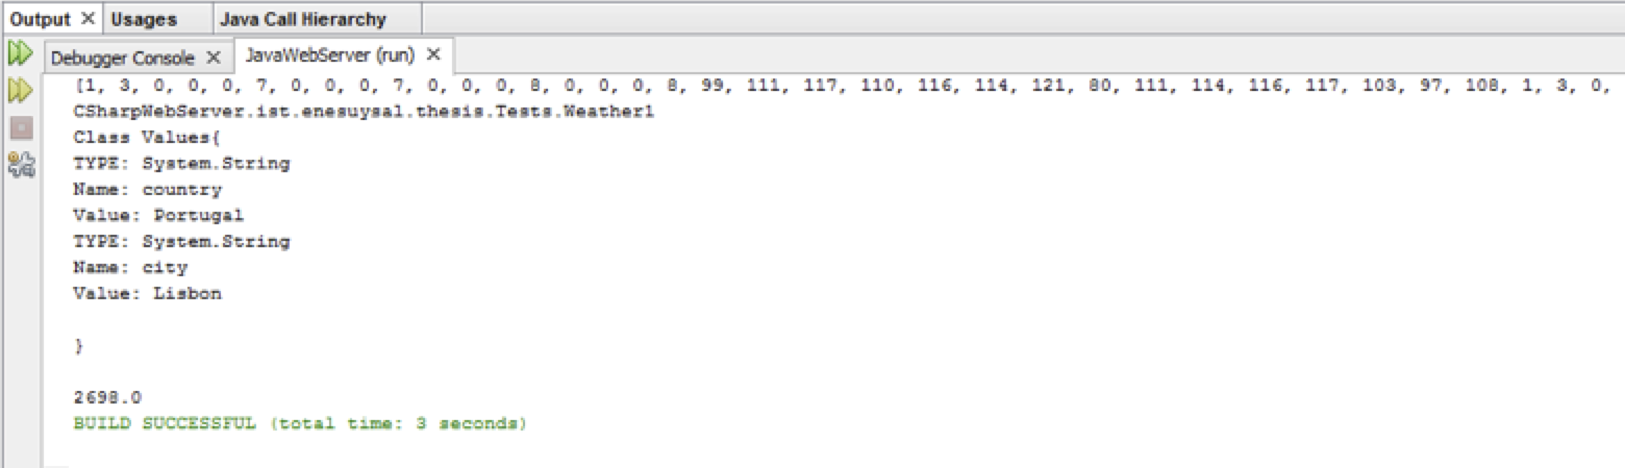
\includegraphics[width=0.9\textwidth]{Figures/scenario4.png}
  \caption[The result of Scenario 1,3 and 4 execution.]{The result of Scenario 3 and 4 execution.}
  \label{fig:scenaro3}
\end{figure}

Scenario 2:

In that scenario, everything is very similar to previous scenario except in {\tt Weather} class has a different value of city which is Braga instead of Lisbon as seen in Listing~\ref{lst:weatherobject2}. In that case the result will be not be same as previous. Since city field is a mandatory field then Weather object will not mapped with {\tt Weather1} class as in as seen in Figure~\ref{fig:scenaro2} and server will not invoke any operation and response will not be returned to user phone application. But in the future if server adds one method its {\tt Receiver} class such as {\tt Weather3} class as seen Listing~\ref{lst:Weather3Ob} with city name is Braga as a defult then without changing anything in the code of your mobile application, mapping will be occur between your mobile applicaion and weathercast provider and result will be returned.

\begin{lstlisting}[caption=Simple weather object class, label=lst:weatherobject2]
          public class Weather
            {
              public String country = "Portugal";
              public String city = "Braga";
            }
\end{lstlisting}

\begin{figure}[!htb]
  \centering
  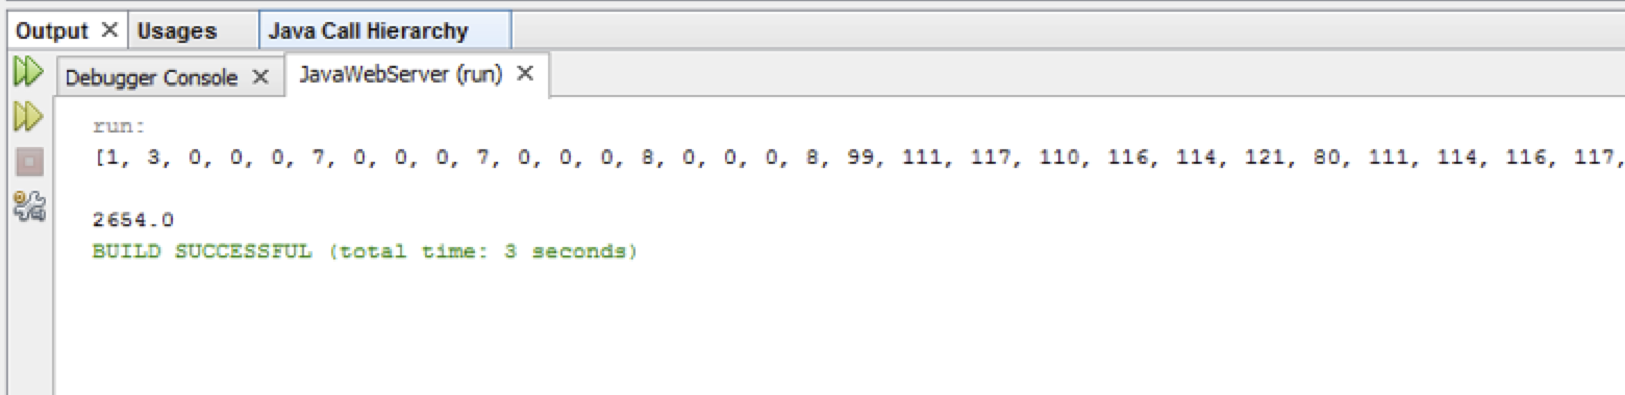
\includegraphics[width=0.9\textwidth]{Figures/scenari2.png}
  \caption[The result of Scenario 2 execution.]{The result of Scenario 2 execution.}
  \label{fig:scenaro2}
\end{figure}

Scenario 3:

Now having another class in {\tt Receiver} class which is called {\tt Weather2} as seen Listing~\ref{lst:Weather2Ob}. {\tt Weather2} has one mondatory field and another one non-mandatory which is optional. Lets send again the same message from mobile phone application as seen in Listing~\ref{lst:weatherobjectv2}. In that case there is a value for country but it is not mandatory. As expected {\tt Weather} object will be mapped to {\tt Weather2} object and server will invoke a operation as seen in Figure~\ref{fig:scenaro3} and response will be returned to user phone application.

\begin{lstlisting}[caption=Weather2 object in Receiver, label=lst:Weather2Ob]
  public class Weather2
    {
      public String country = "Portugal";
      [Mandatory]
      public String city = "Lisbon";
    }
\end{lstlisting}
\begin{lstlisting}[caption=Weather3 object in Receiver, label=lst:Weather3Ob]
  public class Weather3
    {
      public String country = "Portugal";
      [Mandatory]
      public String city = "Braga";
    }
\end{lstlisting}
\begin{lstlisting}[caption=Simple weather object class, label=lst:weatherobjectv2]
          public class Weather
            {
              public String country = "Portugal";
              public String city = "Lisbon";
            }
\end{lstlisting}

Scenario 4:

In that scenario, there are some small changes regarding in Scenario 3. There is no country name as seen in Listing~\ref{lst:weatherobjectv3} , again using {\tt Weather2} class in the {\tt Receiver} where country is non-mandatory. In that case when the message is sent, it will be matched with {\tt Weather2} because country field is not a mandatory field and server will use default value instead of the one in the message. The result will be provided as seen in Figure~\ref{fig:scenaro3} and server will invoke a operation and response will be returned to user phone application.

\begin{lstlisting}[caption=Simple weather object class for Scenario 4, label=lst:weatherobjectv3]
          public class Weather
            {
              public String country = "";
              public String city = "Lisbon";
            }

\end{lstlisting}

As seen in the examples, there is a possibility to have infinity number class in {\tt Receiver} and if the message matches one of them, it runs the operation, returning eventually a result to client. This eliminates data binding parts as stub generation and DOM inspection, because the receiver needs only to be concerned with the interface it which is defined at compile time. Mapping between the message and the formal argument of the receiver method is done in binary, automatically and based on compliance.

%%%%%%%%%%%%%%%%%%%%%%%%%%%%%%%%%%%%%%%%%%%%%%%%%%%%%%%%%%%%%%%%%%%%%%%%
%\section{No static data binding}
%\label{section:noDataBinding}
The  idea is eliminating the need for static data binding (generation of stubs based on a schema). The {\tt Receiver} has always a default value for the message, and only the message components that comply with what the receiver expects are assigned to the matching receiver argument's components. Matching is done by name. This means that the argument is either primitive (int, bool, string) or structured, with named components. Matching is either the same type (primitive types) or name (if the argument is a structured type). Only the components that match are assigned to the formal argument of the operation.

As seen in the example, WSDL file is not necessary or generating a interface based on schema in proposed implementation. Messages do not obey some external schema. Each message has one specific value which are structured or primitive with its own exclusive schema that is nothing more than a self-description, without the value variability that a type exhibits. This value and its description can be validated against an infinite number of schemas, those that have this particular value included in the set of their instances. With using this solution, no longer need to produce a client stub, and that either the client/producer or the server/reader can be changed without breaking interoperability, as longer as compliance (on the client side) and conformance (on the server side) are respected.

%%%%%%%%%%%%%%%%%%%%%%%%%%%%%%%%%%%%%%%%%%%%%%%%%%%%%%%%%%%%%%%%%%%%%%%%
%\section{Anotations}
%\label{section:anotations}
To make compliance possible, the formal argument of each operation should also be serialized as seen in the example. These should also support optional components which use the formal argument component if none in the message matches it. Therefore, the serialization methods in the static serialization class should include whether it is optional. The best is for each primitive data type to have two tags, one for mandatory and another for optional. Annotations allow us define tags for primitive data type.
Messages sent use only mandatory values. Serialized formal arguments can use both mandatory and optional.
%%%%%%%%%%%%%%%%%%%%%%%%%%%%%%%%%%%%%%%%%%%%%%%%%%%%%%%%%%%%%%%%%%%%%%%%
